\documentclass{article}
\usepackage{amsmath}
\usepackage{pgfplots}
\pgfplotsset{compat=1.18} % Asegúrate de usar la versión correcta

\title{Modelo de Generaciones Superpuestas y Demanda de Dinero}
\author{}
\date{}

\begin{document}

\maketitle

\section{Restricción Presupuestaria}

Si \( C_{2,t+1} = 0 \), entonces \( C_{1,t} = y \).

Si \( C_{1,t} = 0 \), "y" se usa para comprar dinero:

\begin{equation}
\frac{v_t}{v_{t+1}} \cdot C_{2,t+1} = y \quad (15)
\end{equation}

Por lo tanto:

\begin{equation}
C_{2,t+1} = \frac{v_{t+1}}{v_t} \cdot y \quad (16)
\end{equation}

\(\frac{v_{t+1}}{v_t}\) representa la tasa real de retorno del dinero fiduciario, es decir, cuántas mercancías pueden ser obtenidas en el período \( t+1 \) si una unidad del bien es vendida por dinero en el período \( t \).

Para una tasa de retorno dada para el dinero \( \frac{v_{t+1}}{v_t} \), podemos obtener los valores óptimos de \( C^*_{1,t} \) y \( C^*_{2,t+1} \) que maximizan la utilidad.

\section{Retorno del Dinero}

El valor en \( t \) depende de lo que se crea que va a valer en \( v_{t+1} \) y así sucesivamente. Depende de una cadena de expectativas acerca del futuro valor del dinero.

Cualquiera que sea la visión sobre el futuro, un parámetro de comparación puede ser el caso en que la visión es la misma para cada generación. Si esta visión sobre el futuro también es la misma de generación en generación, los individuos reaccionarán de igual forma.

\begin{equation}
C_{1,t} = C_1, \quad C_{2,t} = C_2 \quad (17)
\end{equation}

Suponiendo mercados competitivos y teniendo en cuenta las ecuaciones (17) que implican un equilibrio estacionario, y asumiendo "perfect foresight", el precio o valor del dinero será el que iguala la demanda con la oferta.

La demanda de dinero en este modelo será el número de bienes que cada uno elige para vender por dinero, lo cual iguala a los bienes de la dotación inicial que no se consume.

\begin{equation}
y - C_{1,t} \quad (18)
\end{equation}

La demanda total de dinero de la economía será igual a:

\begin{equation}
N_t \cdot (y - C_{1,t}) \quad (19)
\end{equation}

\section{Condición de Equilibrio del Mercado de Dinero}

La oferta total de dinero en pesos es \( M_t \), mientras que expresada en bienes es igual a:

\begin{equation}
v_t \cdot M_t \quad (20)
\end{equation}

La condición de equilibrio del mercado de dinero es:

\begin{equation}
v_t \cdot M_t = N_t \cdot (y - C_{1,t}) \quad (21)
\end{equation}

A partir de esta condición de equilibrio, podemos concluir que:

\begin{equation}
v_t = \frac{N_t \cdot (y - C_{1,t})}{M_t} \quad (22)
\end{equation}

En \( t+1 \) esta relación será:

\begin{equation}
v_{t+1} = \frac{N_{t+1} \cdot (y - C_{1,t+1})}{M_{t+1}} \quad (23)
\end{equation}

Relacionando las ecuaciones (22) y (23) obtenemos lo siguiente:

\begin{equation}
\frac{v_{t+1}}{v_t} = \frac{N_{t+1} \cdot (y - C_{1,t+1})}{M_{t+1}} \div \frac{N_t \cdot (y - C_{1,t})}{M_t} \quad (24)
\end{equation}

En equilibrio estacionario, \( C_{1,t} = C_1 \) y \( C_{2,t} = C_2 \) para todo \( t \), entonces:

\begin{equation}
\frac{v_{t+1}}{v_t} = \frac{N_{t+1}}{M_{t+1}} = \frac{N_t}{M_t} \quad (25)
\end{equation}

Asumiendo que \( N_{t+1} = N_t \) y con una oferta de dinero constante en el tiempo, \( M_{t+1} = M_t \), nos queda:

\begin{equation}
\frac{v_{t+1}}{v_t} = 1 \quad (26)
\end{equation}

Lo que implica que el valor del dinero es constante, y por ende, el nivel de precios también es constante a lo largo del tiempo:

\begin{equation}
v_t = \frac{1}{P_t} \quad (27)
\end{equation}


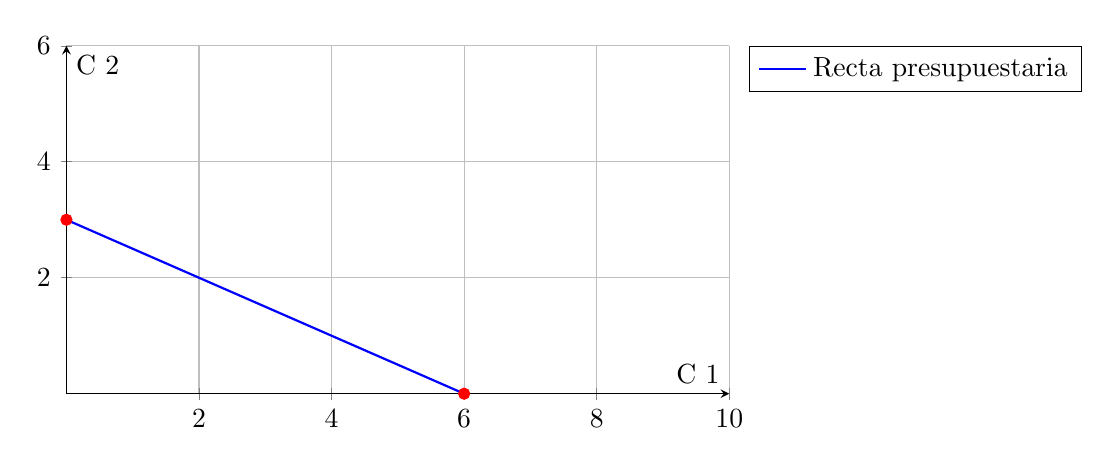
\begin{tikzpicture}
    \begin{axis}[
        axis lines=middle,
        xlabel={C 1},
        ylabel={C 2},
        xmin=0, xmax=10,
        ymin=0, ymax=6,
        domain=0:10,
        legend pos=outer north east,
        grid=both,
        width=10cm,
        height=6cm,
    ]
        % Recta presupuestaria
        \addplot[
            color=blue,
            thick
        ]
        { 3- x/2}; % La ecuación de la recta presupuestaria

        \addlegendentry{Recta presupuestaria}

        % Opcional: marcar los puntos de intersección con los ejes
        \addplot[
            color=red,
            only marks,
            mark=*
        ]
        coordinates {(0, 3) (6, 0)};
        
        % Etiquetas en los puntos de intersección
        \node at (axis cs:0,6) [anchor=south] {$(0, 6)$};
        \node at (axis cs:10,0) [anchor=west] {$(10, 0)$};
    \end{axis}
\end{tikzpicture}

\end{document}
